
\section{Convection Schemes}
\subsection{Introduction}
The convective scheme is responsible for calculating the velocities of all Discrete Vortex Elements given the velocity fields induced by all other elements. The velocity field due to a vortex at any given point is given by the Biot-Savart law, shown in equation \ref{eq:convbase1}

\begin{equation}
\label{eq:convbase1}
\vec{V}(x,y,z)=\frac{\Gamma}{4\pi}\int_{+\infty}^{-\infty} \frac{d\vec{\ell}\times\vec{r}}{|\vec{r}|^3}
\end{equation}

To calculate the velocity field at any given point, the influence of all vortex elements must be taken into account, this is found via the summation of the influences of all elements (representing filaments) found through the Biot-Savart law. This is represented in equation \ref{eq:convbase2} where $N$ is the total amount of elements, and $n$ is the individual element being considered

\begin{equation}
\label{eq:convbase2}
\vec{V}(x,y,z)=\sum_{n=1}^{N} \frac{\Gamma}{4\pi}\int_{+\infty}^{-\infty} \frac{d\vec{\ell_n}\times\vec{r_n}}{|\vec{r_n}|^3}
\end{equation}

The computational cost of a single evaluation of the Biot-Savart law does not change meaningfully for different variables input into equation \ref{eq:convbase1}, the maths required is constant but slight variations may arise from larger inputs. Hence, making the assumption that the computational cost of a single evaluation of the Biot-Savart law is constant, we can express the computational cost as in equation \ref{eq:convbase3} where $C_{Inv}(x,y,z)$ is the computational cost due to a single element at a given point and $A$ is a constant.

\begin{equation}
\label{eq:convbase3}
C_{Single}(x,y,z)=A
\end{equation}

From the expression in equation \ref{eq:convbase3} we can form an expression for the velocity field induced by all elements, this is shown in equation \ref{eq:convbase4}

\begin{equation}
\label{eq:convbase4}
C_{Total}(x,y,z)=\sum_{n=1}^{N} C_{Inv}(x,y,z)=NA
\end{equation}

From equation \ref{eq:convbase4} it can be seen that the complexity of calculating the velocity field is linearly proportional to the amount of elements present. The velocity of an element is found by evaluating the velocity field at that elements position. A single iteration of the convection scheme must calculate the velocity of all elements present, an expression for the computational cost is given in equation \ref{eq:convbase5}

\begin{equation}
\label{eq:convbase5}
C_{Iteration}=\sum_{n=1}^{N} C_{Total}(x_n,y_n,z_n)\approx AN^2
\end{equation}

Equation \ref{eq:convbase5} shows that the computational cost of calculating the new velocities of all elements present increases in complexity proportional to $N^2$. This is known mathematically as an N-Body problem. The computational cost of a single evaluation of the Biot-Savart law, A, is fixed. However modifying the way in which the law is applied constitutes the basis for more computationally efficient convective schemes.
\\\\
In this section, two modifications to the convective scheme are suggested and evaluated. Both schemes necessarily introduce errors into the numerical solution. The schemes are evaluated based upon a consideration of their performance and accuracy

\subsection{Biasing}
Biasing is the simplest method of optimization for the convection scheme. Biasing works by "biasing" which elements are taken into account when convecting a given element. Consider again the Biot-Savart law, shown in equation \ref{eq:bias1} for clarity.

\begin{equation}
\label{eq:bias1}
\vec{V}(x,y,z)=\frac{\Gamma}{4\pi}\int_{+\infty}^{-\infty} \frac{d\vec{\ell}\times\vec{r}}{|\vec{r}|^3}
\end{equation}

From equation \ref{eq:bias1} two things can be noted, the influence of an element on a given element is majorly dependent only on two variables, the convecting elements vorticity $\Gamma$ and the its distance vector $\vec{r}$. Biasing methods exploit these relationships by ignoring the convective effects of an element if its influence on a certain element can be considered negligible. 
\\\\
Determining whether or not an elements influence is negligible requires an evaluation of either the vorticity $\Gamma$ or distance vector $\vec{r}$ of the given element, or a coefficient based upon both of these. This evaluation must be performed for all elements every time an element is convected, so the evaluation must be performed $N^2$ times per iteration, an equal amount of times as the Biot-Savart law must be evaluated in the absence of a biasing scheme. It is also important to note that this evaluation process must be performed even for elements whose effects will be taken into account. The evaluation scheme must therefore be kept lightweight and efficient in order to pose a performance increase of the scheme. If a computationally costly evaluation process is used it may pose a decrease in both overall performance and accuracy of the simulation.
\\\\
The simplest biasing system would make an evaluation based upon both Vorticity and distance vector, such an evaluation is shown in the condition in equation \ref{eq:bias2} where A is an arbitrary constant.

\begin{equation}
\label{eq:bias2}
\frac{\Gamma}{\vec{r}}>A
\end{equation}

This approach provides the most accurate results, however it is also the most computationally expensive as it involves both an evaluation and a calculation. Two other criteria may be used for biasing the effect of elements based solely on distance and vorticity respectively. Evaluations based on on either vorticity or distance have the advantage of being more lightweight and representing an almost negligible overhead Whether it is best to consider vorticity or distance depends on the situation that need be modeled. A situation where all elements are close would likely benefit more from an evaluation based on vorticity, however an application where elements are spaced with a larger distance may benefit from an evaluation based on distance.
\\\\
The simulation considered here is of a wake. This involves initially closely spaced elements seeded with initial values along the wing of an aircraft. As the simulation progresses more elements are spawned in rows, the distance between early rows and later rows increases linearly as more rows are spawned. As there is a large distance between elements in the simulation, a distance based biasing method is appropriate. New rows of elements are created when the distance between the bound elements and the last seeded free elements reaches a limit, from this a grid with near-uniform spacing is created. Thus, the computation cost for convecting an individual element is given by equation by equation \ref{eq:bias3} where B refers to the amount of elements present when the grid is sufficiently large such that elements are spread over a distance where the distance based evaluation is met.
\begin{equation}
\label{eq:bias3}
C_{Total(x,y,z)}=\begin{cases}
    NA       & \quad N<B\\
    BA  & \quad N>B\\
  \end{cases}
\end{equation}

In equation \ref{eq:bias3} it can be seen that the computational cost for a given element is seen to reach a maximum value and remain constant. If the grid is sufficiently large such that this condition becomes true, the computational cost is given by equation \ref{eq:bias4}

\begin{equation}
\label{eq:bias4}
C_{Iteration}=\sum_{n=1}^{N} C_{Total}(x_n,y_n,z_n)=NBA
\end{equation}

From equation \ref{eq:bias4} it is apparent that if a well designed clustering scheme is implemented the N-Body problem reduces in complexity from $ON^2$ to $ON$.

\subsection{Clustering Schemes}
\subsubsection{Introduction}
Clustering schemes assume that the effect of certain elements on a given element may be "clustered" and approximated to the effect of one element of an equivalent strength and position. By clustering elements together their influence can be taken into account with only one iteration of the Biot-Savart law, this reduces computational overhead. An example of this is shown in Figure \ref{fig:StoC}, where in situation A the leftmost element is convected by a series of distant but closely spaced element. In situation B, the  series of disant but closely spaced elements are approximated to a single element.

\begin{figure}[H]
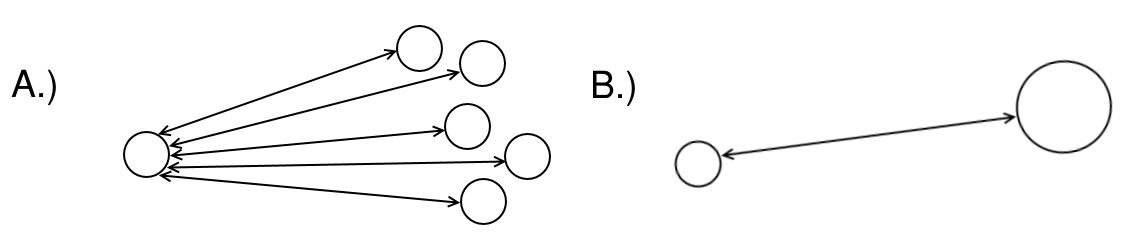
\includegraphics[width=1.0\textwidth]{Figures/SeriesToCluster.png}
\caption{\label{fig:StoC}Distant Elements Approximated to a Single Cluster}
\end{figure}

The series of elements approximated to a single element in Figure \ref{fig:StoC} is only valid when the convection of the leftmost element is to be performed. For example, the cluster grouping shown could not be used to convect an element inside the cluster group. Hence every element represents a unique situation with its own unique cluster groupings. However, the calculation of these unique cluster groupings represents a large computational overhead, and thus is not beneficial as a method of optimization.
\\\
To overcome the large computation overhead associated with calculated unique cluster groupings a method is used where the cluster groupings are selected based upon which cluster groups are applicable to most elements. For example, consider figure \ref{fig:ThreeClusters}. Here 3 sets of closely spaced elements can be seen, clustered into the groups A,B and C.

\begin{figure}[H]
\centering
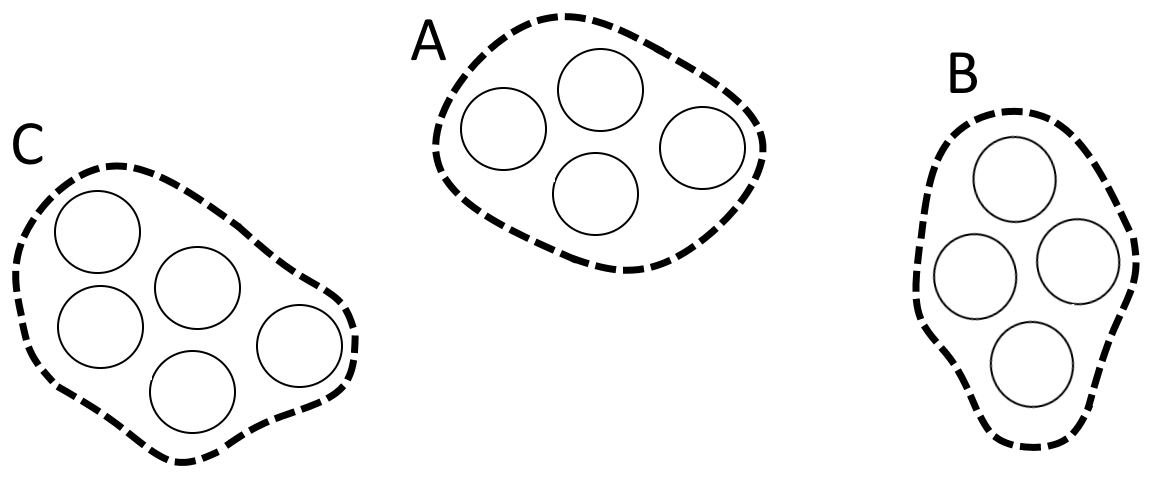
\includegraphics[width=0.6\textwidth]{Figures/ThreeClusters_Example.png}
\caption{\label{fig:ThreeClusters}Closely Spaced Elements and their Respective Cluster Groupings}
\end{figure}

Of course, these cluster groups cannot be used to convect any of the elements, as all elements are in clusters. However, when a single element is to be convected, it could be convected with all elements in its own cluster, and all clusters except its own. This way every element is convected by every other element either directly or through a cluster. Consider for example an element inside cluster B, its convection in this manner is demonstrated in figure \ref{fig:EinB}

\begin{figure}[H]
\centering
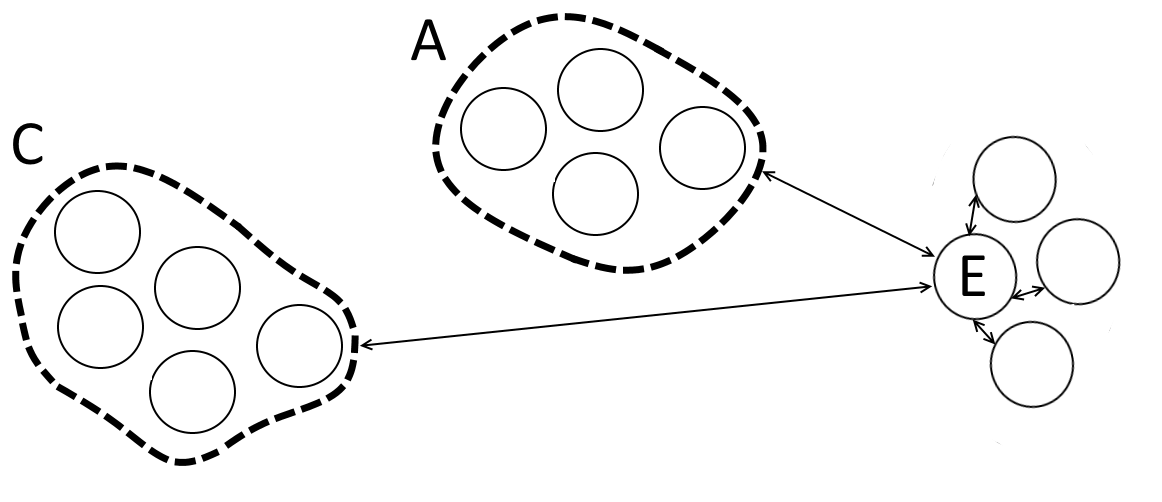
\includegraphics[width=0.6\textwidth]{Figures/ElementInB.png}
\caption{\label{fig:EinB}Element 'E' in cluster 'B' Convecting with Individual Elements and Clusters}
\end{figure}

In figure \ref{fig:EinB} an element "E" from cluster B is shown being convected in the previously discussed way. Consider all elements in cluster C, if they are convected in this manner they will be convected by clusters A and B. Hence, the elements in B and A will both convect with cluster A. Likewise elements from clusters C and A will have cluster B in common. In this way clusters may be calculated once for all elements and still be applicable, despite each element requiring a unique situation.
\\\\
If clusters A and B were closer together it may not be beneficial to convect individual elements in B with the cluster of A but instead with the individual elements of A. Neither is it necessary to convect the elements in cluster B with cluster A, an evaluation based on distance and vorticity could be made to determine whether it would be best to take into account close clusters as a cluster of their constituent elements.
\\\\
Approximating a series of elements to a cluster imposes a degree of error as those individual elements are assumed to act at the position of the cluster rather than their actual positions.

\subsubsection{Fixed and Dynamic Cluster Scaling}
A fixed cluster scaling scheme is the simplest clustering scheme considered in this report. The scale of the cluster is used here not to refer to the amount of elements in the cluster. The amount of elements in a cluster is determined by the spatial positioning of the elements. Rather, the scale of a cluster refers to the way clusters are combined to create new clusters. Up until this point clusters comprised solely of elements have been considered, however a situation could be  envisaged where with increased distance from a series of clusters, those clusters could be further clustered together to create a cluster comprised of clusters. This is demonstrated in figure \ref{fig:ClustClust} where situation A represents two distant clusters convecting with a given cluster and situation B represents the same situation where the two distance clusters are clustered together.

\begin{figure}[H]
\centering
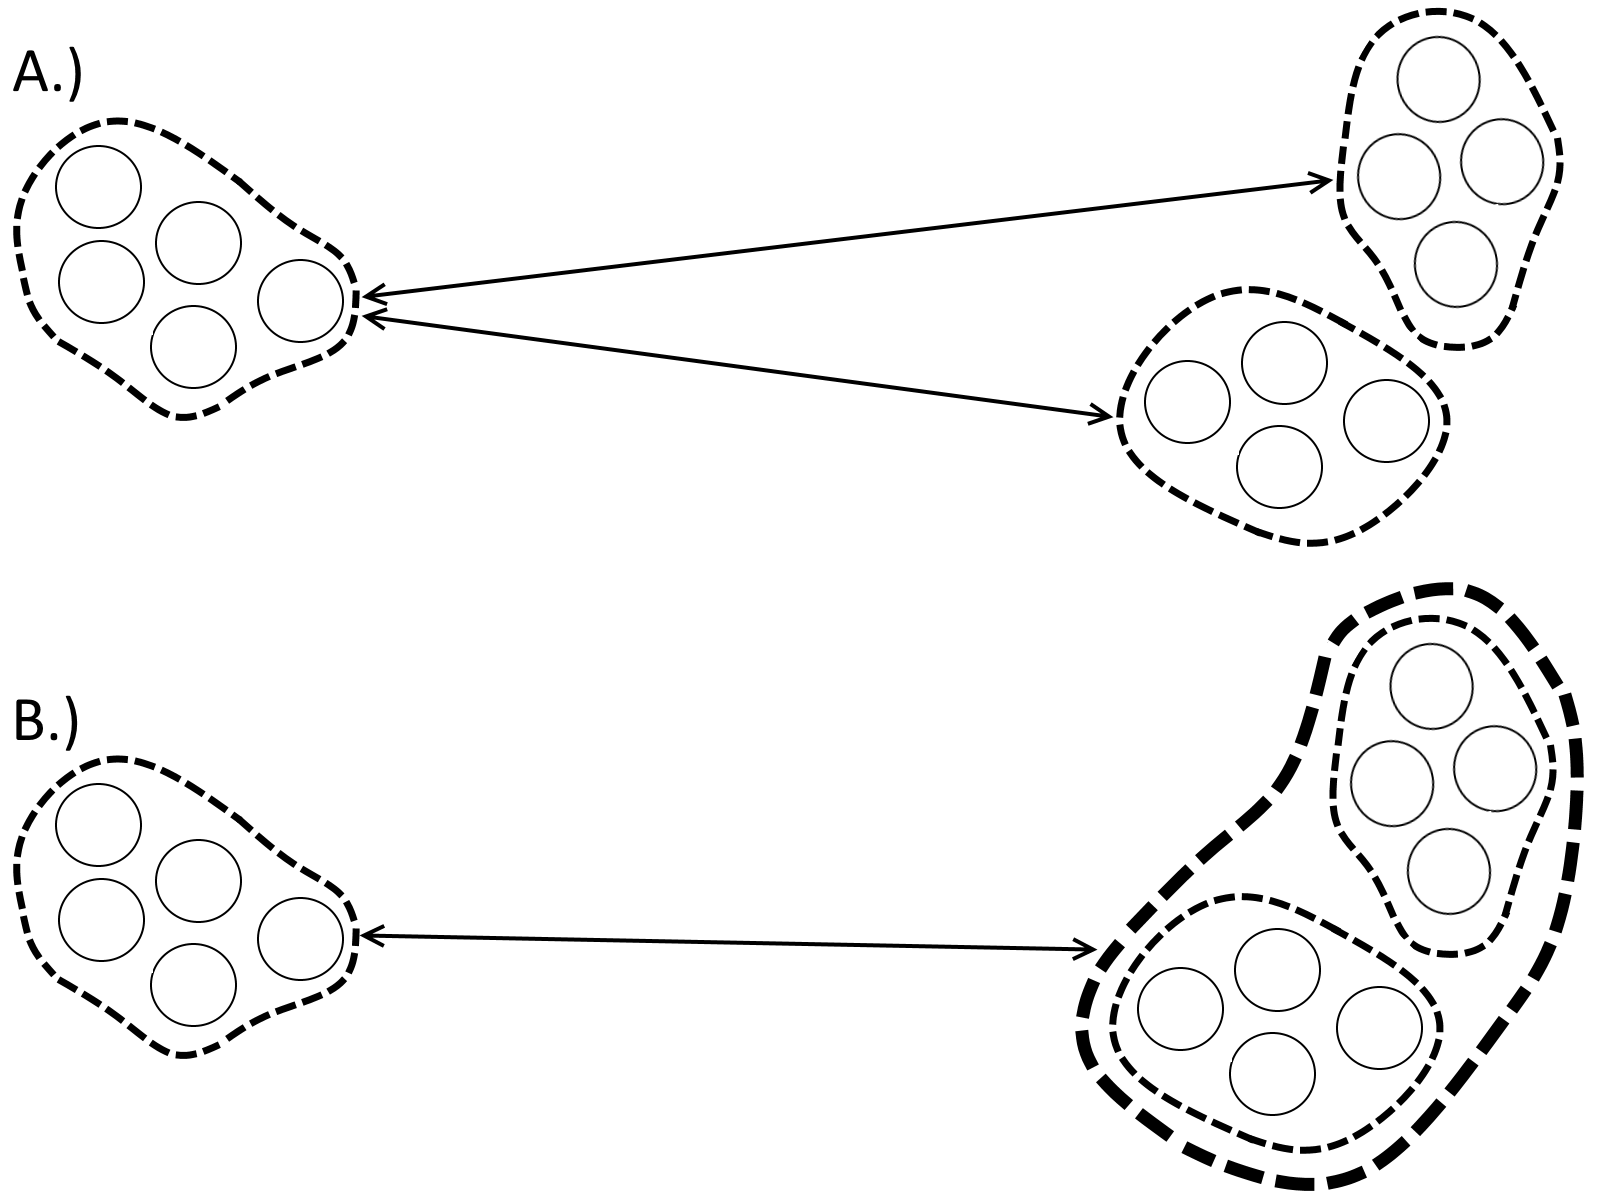
\includegraphics[width=0.55\textwidth]{Figures/ClusterCluster.png}
\caption{\label{fig:ClustClust}Example of Clustering Clusters Together}
\end{figure}

In a fixed cluster scaling scheme clusters are clustered together. Conversely, in a dynamic cluster scaling scheme clusters are clustered together where appropriate to create clusters of clusters.
\\\\
In a fixed cluster scale scheme the clusters are determined via the spatial position of the elements. For the cluster groups to be useful they must be comprised of elements clustered together because they are spatially close together, this gives rise to a physical size of the cluster. In the present simulation, elements are created in a line equidistant to each other and released with uniform velocity perpendicular to the spawn line. Thus the 
elements form a roughly grid shaped pattern as shown in figure.
\\\\
Because the elements form a grid shaped pattern with roughly equal $x$ and $y$ grid spacing the element count in a cluster is fixed, giving rise to the cluster size $N_{Cluster}$. The Biot-Savart law is required to be iterated for all clusters except the cluster the element in question is contained within,  every element from this cluster must be taken into account, the computational cost of convecting a single element is given in equation \ref{eq:clust1}

\begin{equation}
\label{eq:clust1}
C_{Element}=A\frac{N}{N_{Cluster}}+A(N_{Cluster}-1)
\end{equation}

The first term in equation \ref{eq:clust1} represent the computational cost of iterating the Biot-Savart law for all the clusters. Likewise, the second term represents the computation cost of iterating the Biot-Savart law for the individual elements in the element in questions cluster. The computational cost for convecting all elements present is therefore given by equation \ref{eq:clust2}, the term $C_{Cluster}$ is the computational cost of calculating the cluster groupings every loop.

\begin{equation}
\label{eq:clust2}
C_{All}=NA\Big(\frac{N}{N_{Cluster}}+(N_{Cluster}-1)\Big)+C_{Cluster}
\end{equation}

Equation \ref{eq:clust2} can be rearranged to equation \ref{eq:clust3}

\begin{equation}
\label{eq:clust3}
C_{All}=\frac{AN^2}{N_{Cluster}}+AN(N_{Cluster}-1)+C_{Cluster}
\end{equation}

From equation \ref{eq:clust3} it is apparent that the increase in complexity of the scheme still increases proportional to $ON^2$ as in the unclustered case. However the leading term for the fixed scale cluster scheme is proportional to $AN^{-1}_{Custer}N^2$ compared to the unclustered case where complexity rises with $AN^2$. This necesserily represents an optimization, assuming $C_{Cluster}$ is suitable low, as $N_{Cluster}>1$ and in practice takes a value of around 10.

\subsubsection{Cluster Position}
An error is introduced into a simulation using a clustering scheme as the position of every individual element in a cluster is lost and every element assumed to act the clusters potion. Determining the position of the cluster will therefore have an effect of the magnitude of this error. The simplest approach to calculate a clusters position would be to average the coordinates of all elements in the cluster. This method weights the position of all elements equally in a cluster. In this section two alternative methods are discussed, a weighted average and a simpler highest influence approach.
\\\\











